\documentclass[usenames,dvipsnames]{article}
\usepackage[
		papersize={8in,9in},
		]
	{geometry}
\usepackage{tikz}

 \newcommand*\circled[1]{\tikz[baseline=(C.base)]\node[draw,circle,inner sep=1.2pt,line width=0.2mm,](C) {\small #1};}

\usepackage{amssymb} %maths
\usepackage{amsmath} %maths
\usepackage[utf8]{inputenc} %useful to type directly diacritic characters
\usepackage{expex}

\usepackage{ulem}
\begin{document}


  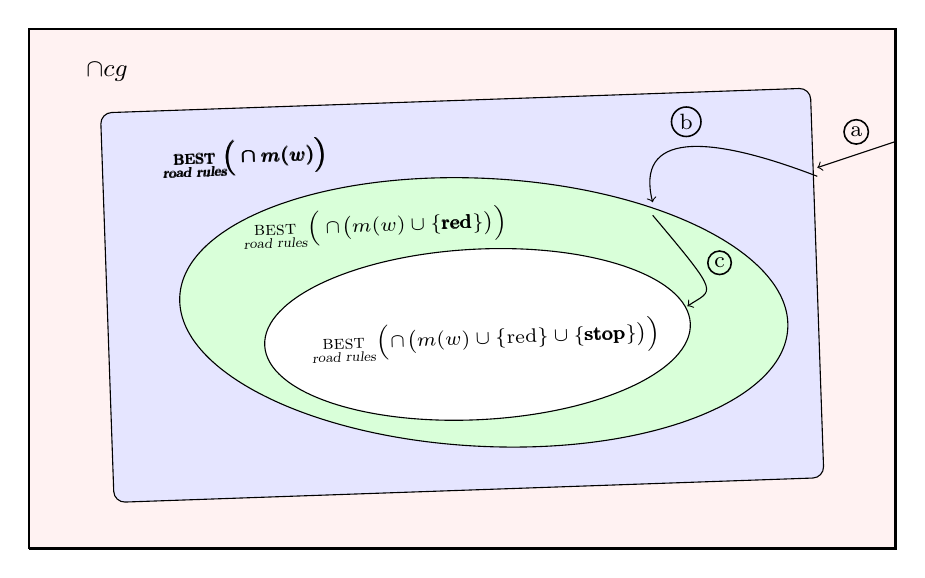
\begin{tikzpicture}[scale=2.2]
    \draw[line width=1pt,fill=red!5] (0,0) -- (5,0) -- (5,3) -- (0,3) -- (0,0);
    \node[align=center] at (.45,2.75) {\small $\cap cg$};
%    \node[align=center] at (4.75,2.75) {\circled{\footnotesize 1}};
    \draw[->] (5,2.35) -- node[above] {\circled{\footnotesize a}} (4.55,2.2) ;
    
    \draw[rotate=2,rounded corners,fill=blue!10] (.5,.25) rectangle (4.6,2.5);
    \node[align=center, rotate=2] at (1.25,2.25) {\scriptsize $\pmb{\underset{\textsl{road rules}}{\textsc{best}}\!\Big(\cap m(w)\Big)}$};
 %   \node[align=center] at (4.30,2.45) {\circled{\footnotesize 2}};
   \draw[->] (4.55,2.15) .. controls (3.9,2.4) and (3.5,2.4) ..  node[above] {\circled{\footnotesize b}} (3.6,2);
    
    \draw[rotate=-3, fill=green!15] (2.55,1.5) ellipse [x radius=50pt, y radius=22pt]; %[postaction={decoration={text along path,    text={${best(\cap(m(w))}${}}}, decorate}] ;
    \node[align=center, rotate=2] at (2,1.85) {{\scriptsize $\underset{\textsl{road rules}}{\textsc{best}}\Big(\cap\!\big(m(w)\cup \{\pmb{\text{red}}\}\big)\Big)$}};
 %   \node[align=center] at (3.8,1.7) {\circled{\footnotesize 3}};
    \draw[->] (3.6,1.925) .. controls (4,1.45) and (3.95,1.5)  .. node[above, xshift=5pt] {\circled{\footnotesize c}} (3.8,1.4) ; 
    
    \draw[rotate=3,fill=white] (2.65,1.1) ellipse [x radius=35pt, y radius=14pt];
    \node[align=center, rotate=2] at (2.64,1.2) {{\scriptsize $\underset{\textsl{road rules}}{\textsc{best}}\Big(\!\cap\!\big( m(w)\cup \{\text{red}\} \cup \{\pmb{\text{stop}}\}\big)\Big)$}};
 %   \node[align=center] at (3.6,1.35) {\circled{\footnotesize 4}};
    
  \end{tikzpicture}
\end{document}